% Created 2019-04-27 Sat 22:37
\documentclass[11pt]{article}
\usepackage[utf8]{inputenc}
\usepackage[T1]{fontenc}
\usepackage{fixltx2e}
\usepackage{graphicx}
\usepackage{longtable}
\usepackage{float}
\usepackage{wrapfig}
\usepackage{rotating}
\usepackage[normalem]{ulem}
\usepackage{amsmath}
\usepackage{textcomp}
\usepackage{marvosym}
\usepackage{wasysym}
\usepackage{amssymb}
\usepackage{hyperref}
\usepackage{array}
\usepackage{titlesec}
\usepackage{titling}
\usepackage{longtable}
\usepackage[margin=0.5in]{geometry}
\titleformat{\section}
{\large \bfseries}
{}
{0em}
{}

\titleformat{\subsection}
{\bfseries}
{}
{0em}
{}[\titlerule]

\titleformat{\subsubsection}
{\bfseries }
{$\bullet$}
{2em}
{}

\tolerance=1000
\author{Jonatan Ahumada\\
Paula Alarcón\\
Thomás Zarrate
}
\date{\today}
\title{Fundación Universitaria Konrad Lorenz \\
Cultura II: Bogotá y sus Historias\\
Taller: graffitis}
\begin{document}

\maketitle
\section{Reflexión}
\label{sec-2}
La importancia que tiene el graffiti en Bogotá radica en su cualidad territorial e invasiva. En otros términos, radica en 
el hecho de que no es posible evadir una discusión sobre el graffiti
en tanto que el fenómeno se proyecta desde el mismo espacio urbano
que habitamos colectivamente. Por este motivo, la discusión 
sobre el graffiti no encaja en la misma categoría que una discusión 
acerca de otro tipo de 'bellas artes' solo por el hecho de ser 
una forma pictórica, sino que en sí mismo trae a colación preguntas
sobre el adecuado uso de espacio urbano y de los discursos que las 
diferentes facciones de graffiteros consignan al imaginario público.

Un aspecto que nos ha llamado la atención del graffiti en Bogotá es 
su popularización entre el gremio de los diseñadores gráficos. Tanto 
así que se mencionó como una característica del \emph{street art} que marca
una distinción importante entre este y el graffiti como tal. Ahora,
los graffiteros, en este momento histórico, no son representantes de sectores sociales con
problemáticas claramente definidas según algún marco teórico, como alguna vez lo fueron (por ejemplo, el
racismo, el narcotráfico, la lucha de clases, etc). 

Por el contrario, ahora son por
decirlo de algún modo, 'profesionales de la insurrección' o, según la expresión más frecuente, fueron
"absorbidos por el centro" dentro de una dinámica centro-periferia. Tienen, 
por ejemplo, páginas web, son subsidiados por el estado y se estudian 
en aulas de clase. Es bastante irónico en el sentido en que Octavio 
Paz describe la ironía en el arte (se parodia y se niega a sí misma). Solo que en el graffiti tiene la
cualidad (o el agravante), de que no es solo una cuestión de arte, 
sino una cuestión política. 

Un ejemplo de esta ironía:  a medida que los murales de colores vibrantes maquillan los edificios
de la ciudad, menos se verán los graffitis del estilo "Uribe
asesino". O, por ejemplo, el hecho de que Justin Bieber fuera escoltado
por la policía a graffitear cuando a poco mataron a un jóven. Lo podríamos llevar a mayor extremo:
por ejemplo, que los mensajes ambientalistas estén hechos precisamente con spray o, más aún,
la esperanza de producir un cambio pintando paredes.  	


\section{Cuadro Comparativo}
\label{sec-1}
\begin{center}
\begin{longtable}{|c|p{4cm}|c|p{4cm}|}
\hline
Street Art & Desc. & Graffiti & Desc.\\
\hline
\raisebox{-\totalheight}{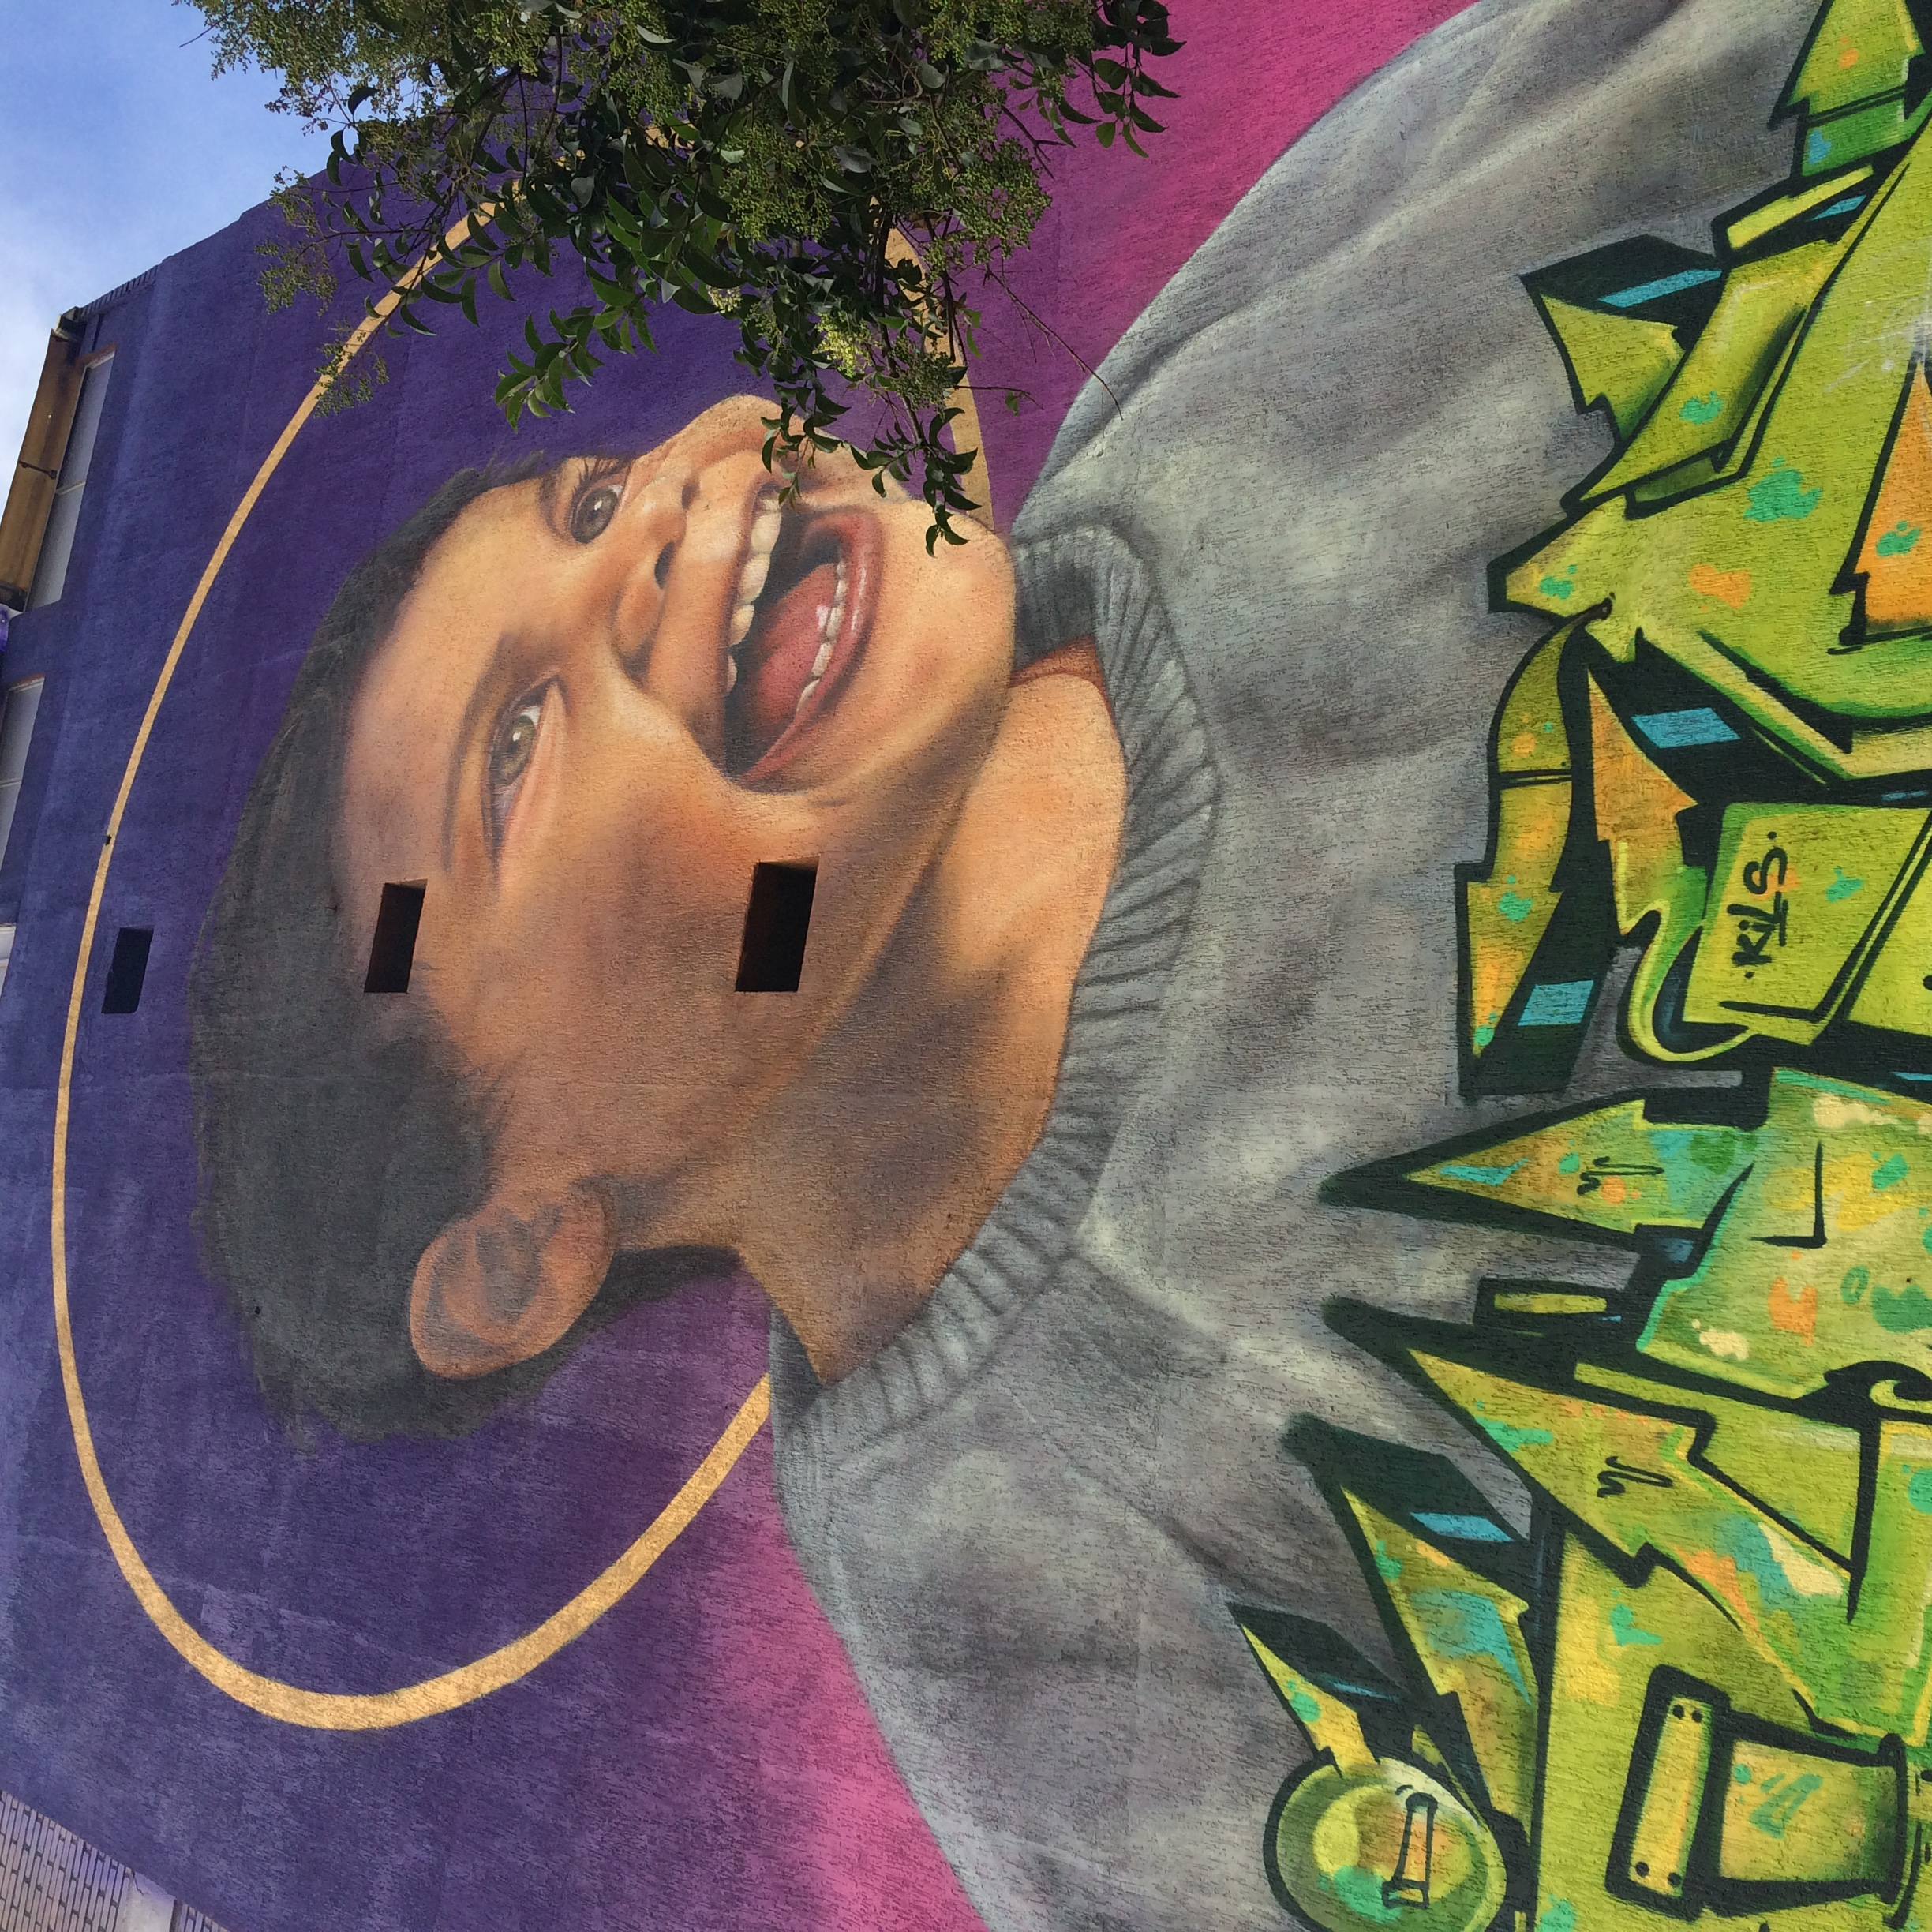
\includegraphics[width=.25\linewidth, angle=270,origin=c]{./graffitti/ninio.JPG}} & \begin{itemize}
 \item complejidad + dimensiones 
 \item probablemente un colectivo
 \item estilo realista + lettering
 \item diálogo entre estéticas 
 \end{itemize}	


&\raisebox{-\totalheight}{ 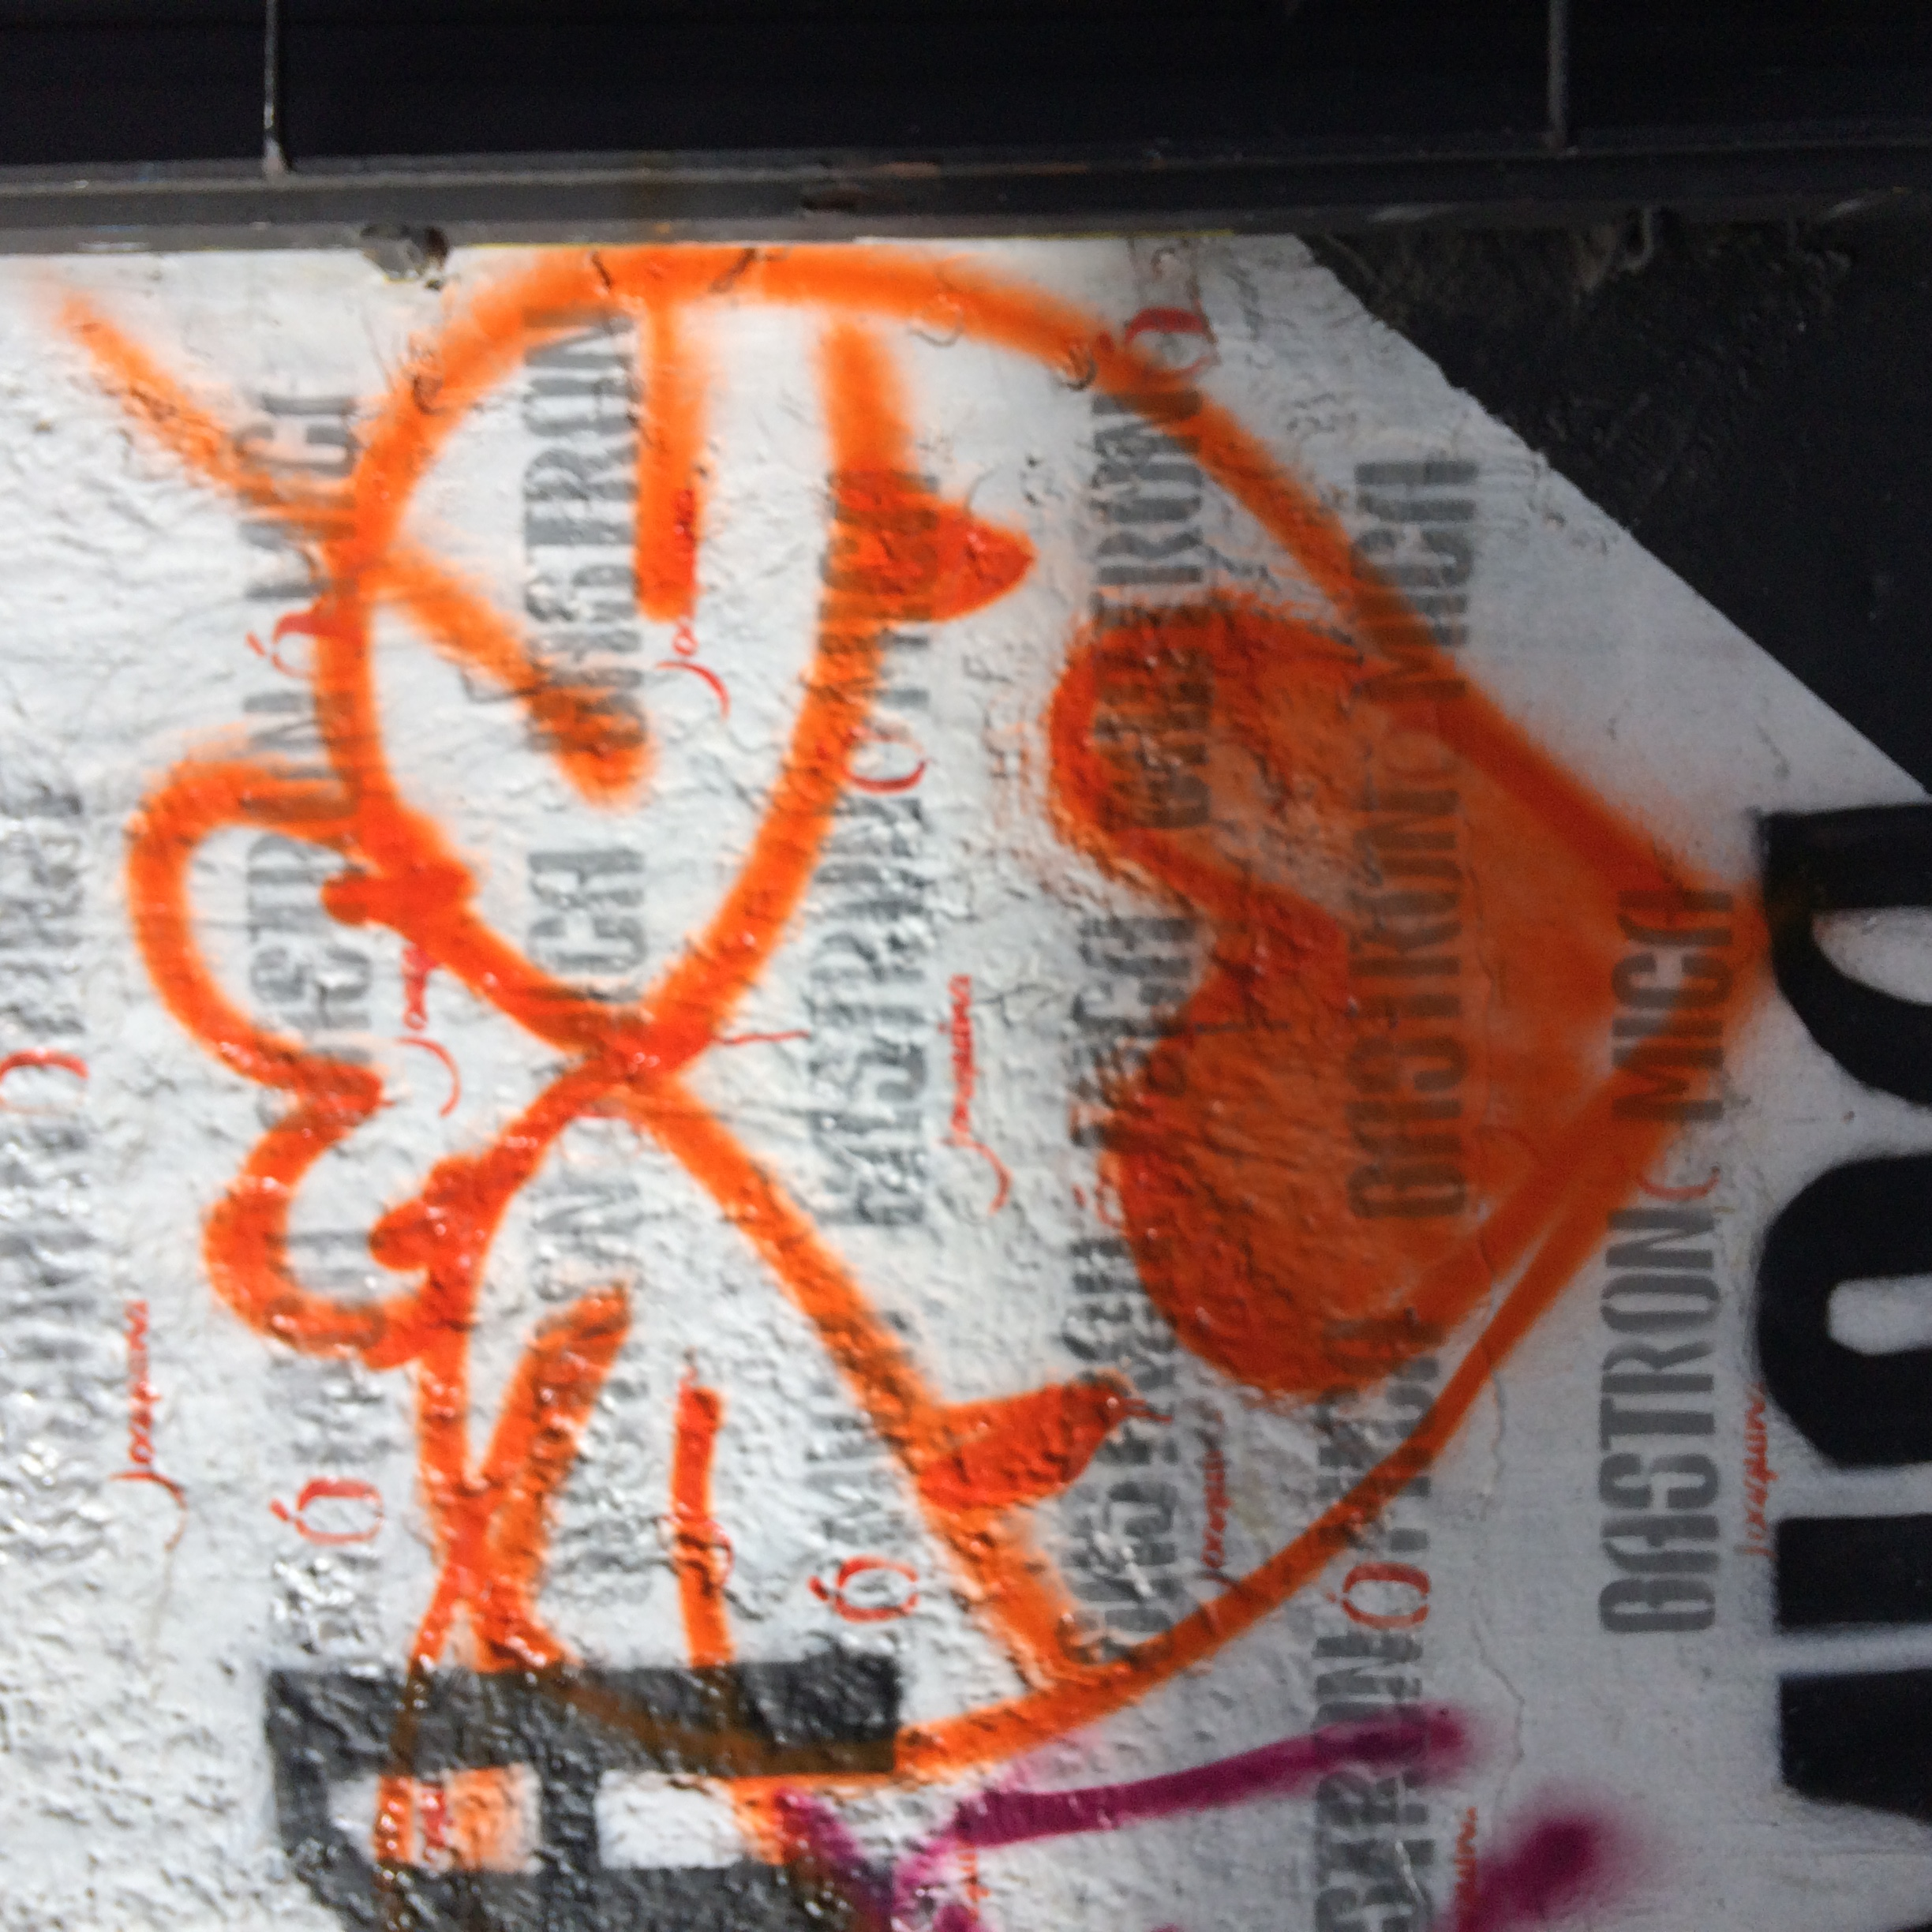
\includegraphics[width=.25\linewidth, angle=270,origin=c]{./graffitti/gffti1.JPG}} &

 \begin{itemize}
 \item  ejemplo de tag
 \item  es incomprensible
 \item se nota la rapidez
 \item diálogo entre estéticas 
 \end{itemize}	
 \\
\hline
\raisebox{-\totalheight}{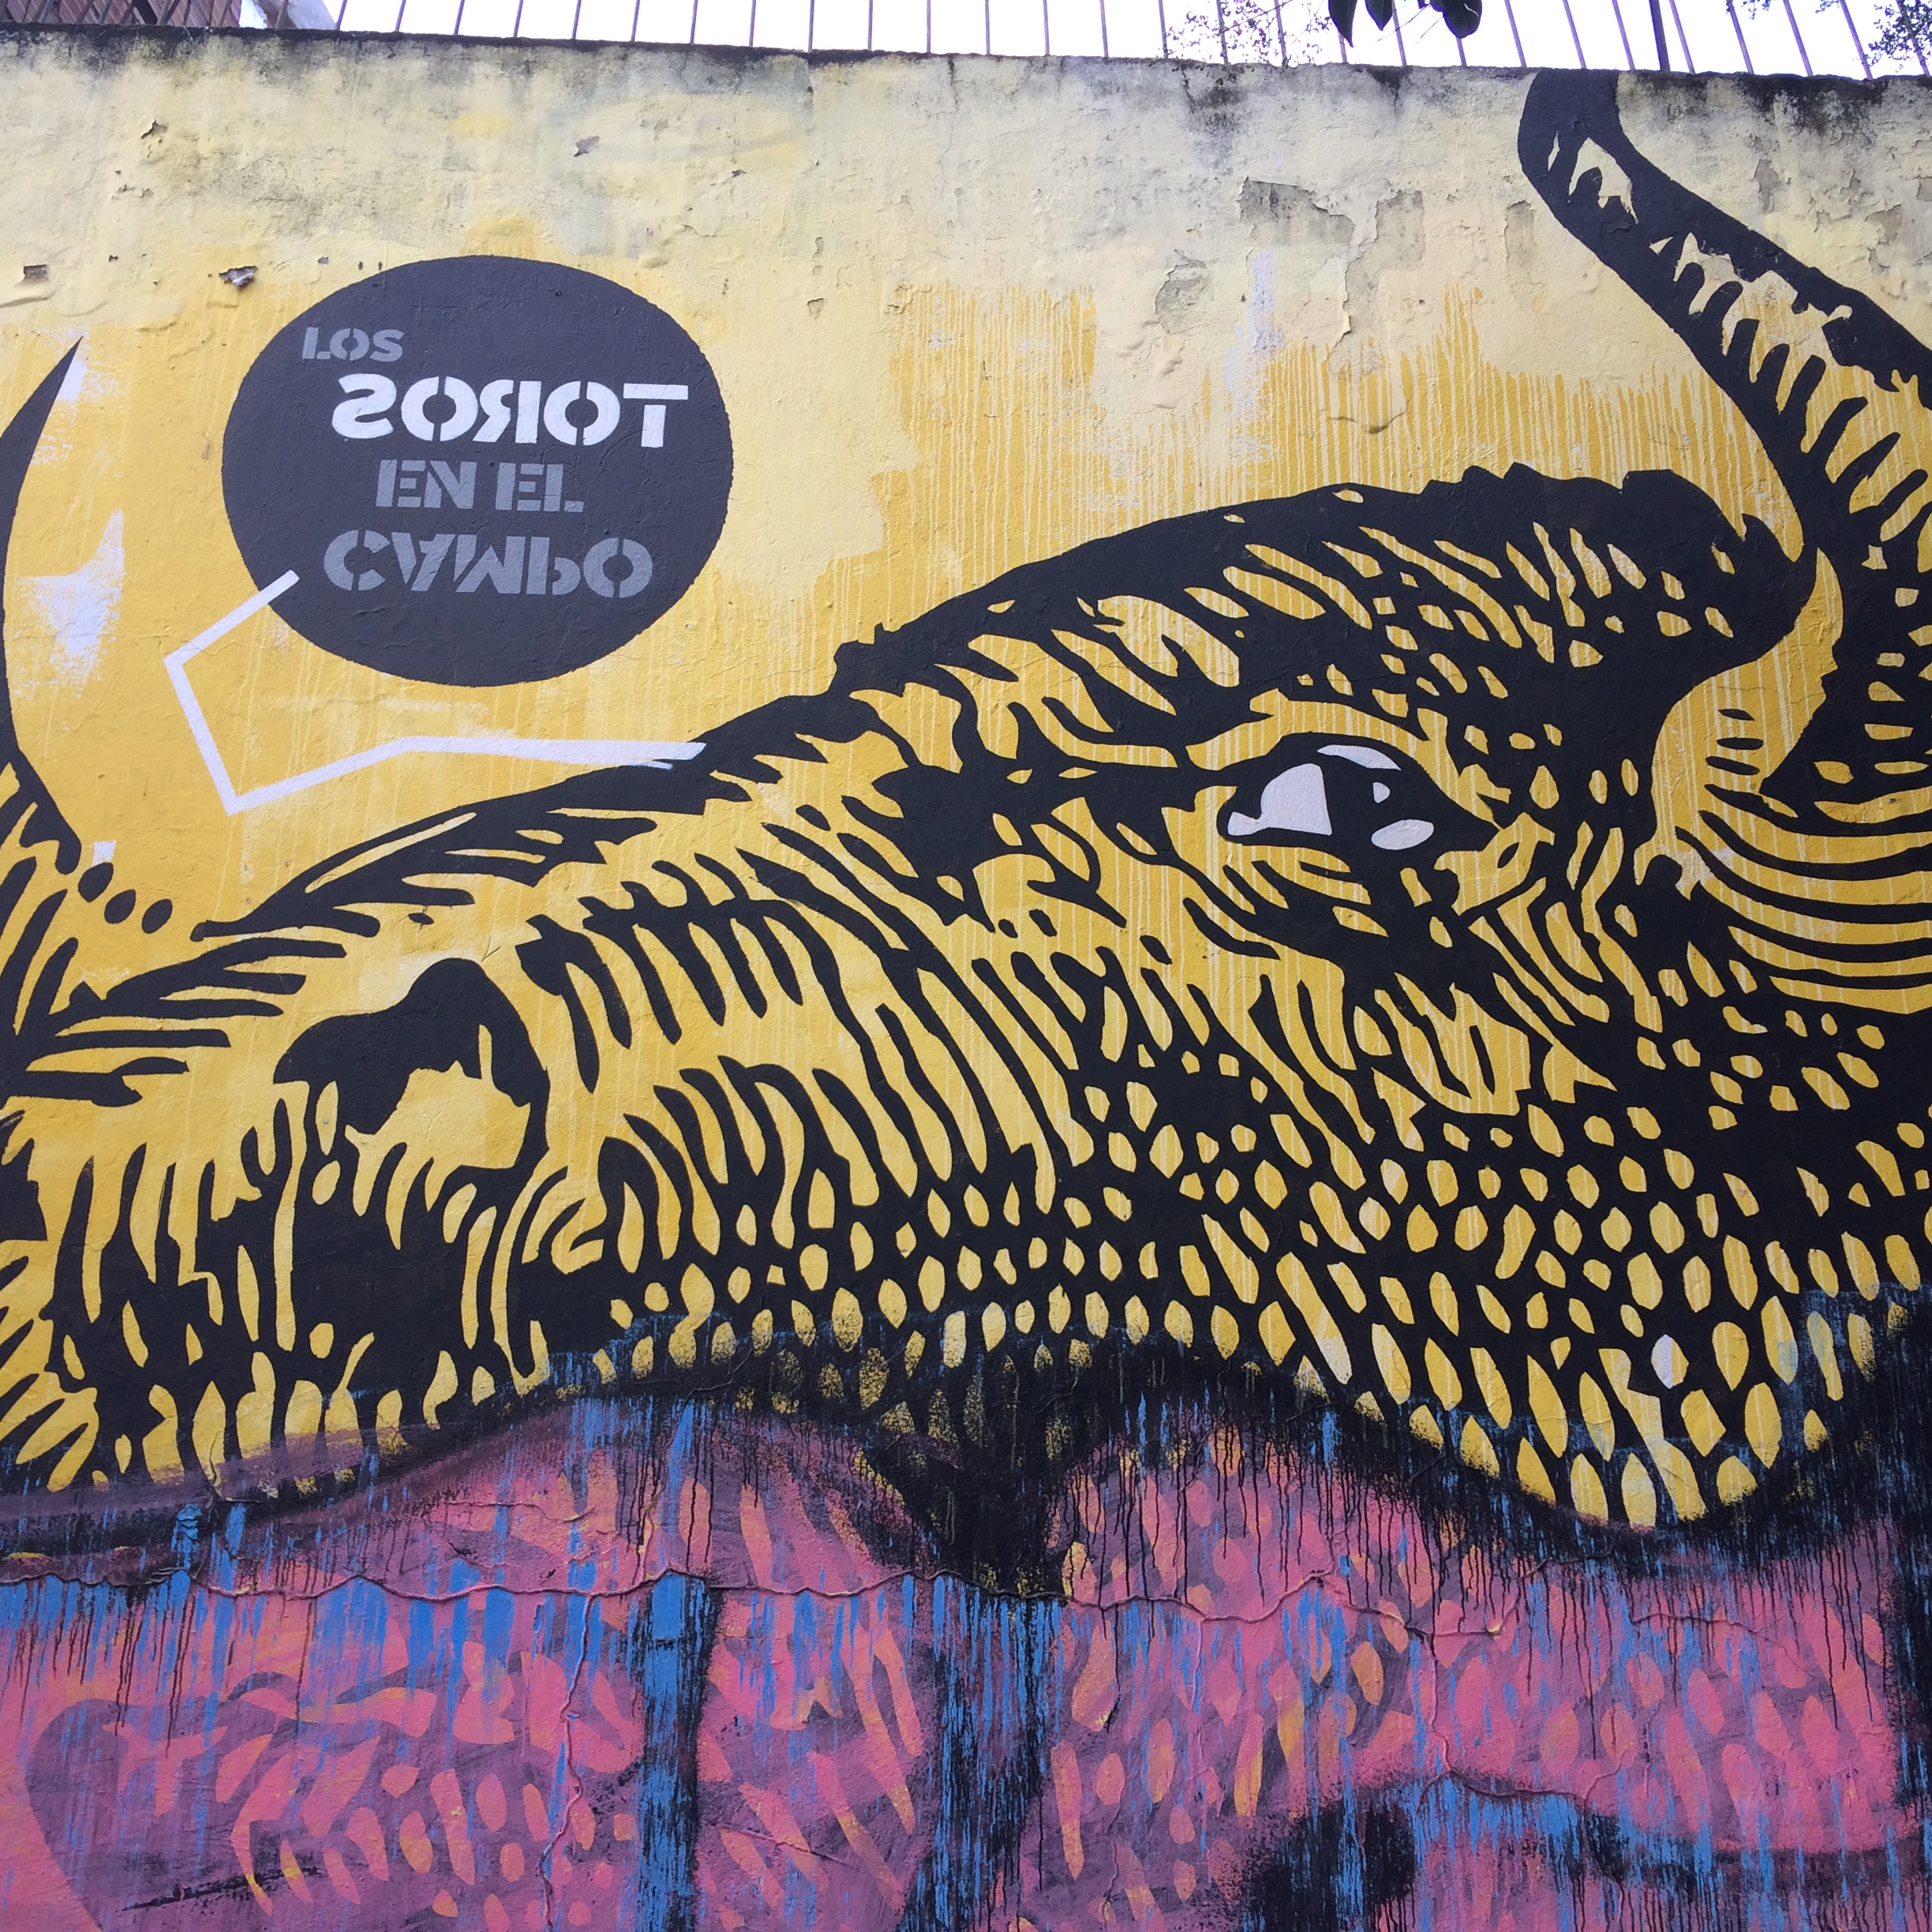
\includegraphics[width=.25\linewidth, angle=0,origin=c]{./graffitti/toro.JPG}} & 
\begin{itemize}
 \item usa stencil
 \item nombre del colectivo
 \item reflexión social
 \item fondo también es en stencil (elaborado)
 \end{itemize}	

&\raisebox{-\totalheight}{ 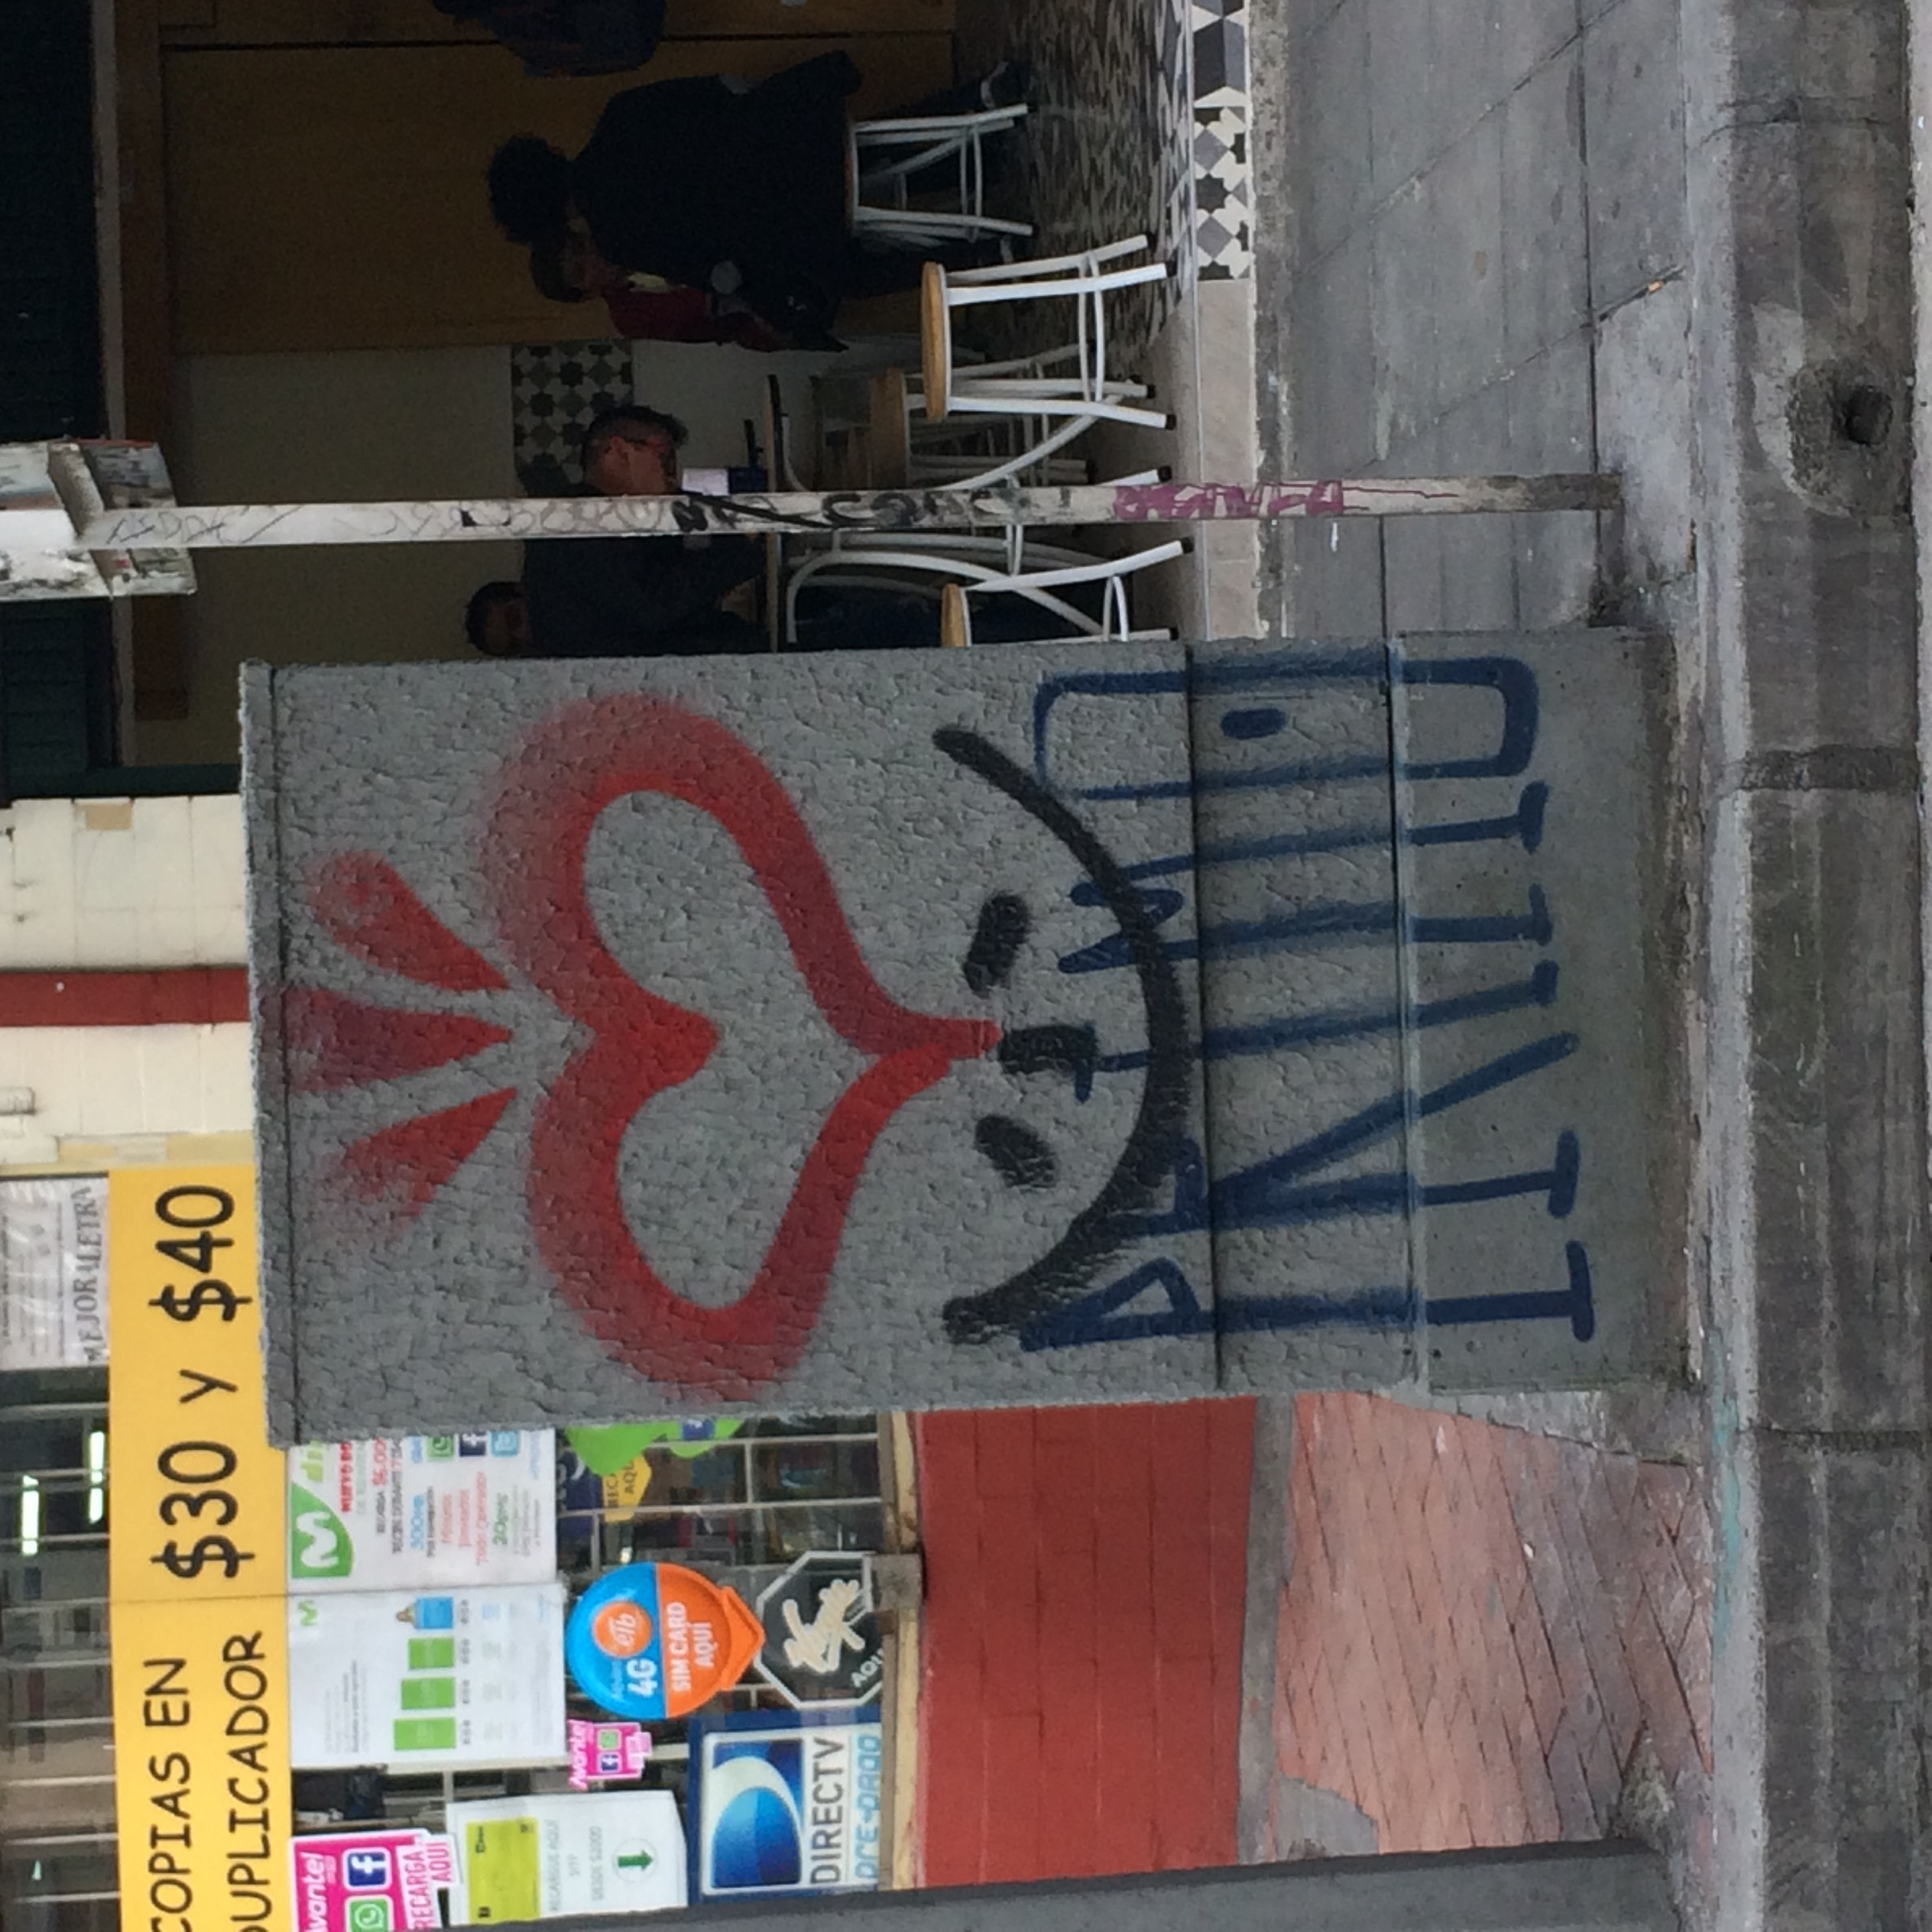
\includegraphics[width=.25\linewidth, angle=270,origin=c]{./graffitti/gffti2.JPG}} & \begin{itemize}
 \item demarcación del territorio (teléfono)
 \item nombre o trag legible o claro ("Primo")

 \end{itemize}	
 \\
\hline
\raisebox{-\totalheight}{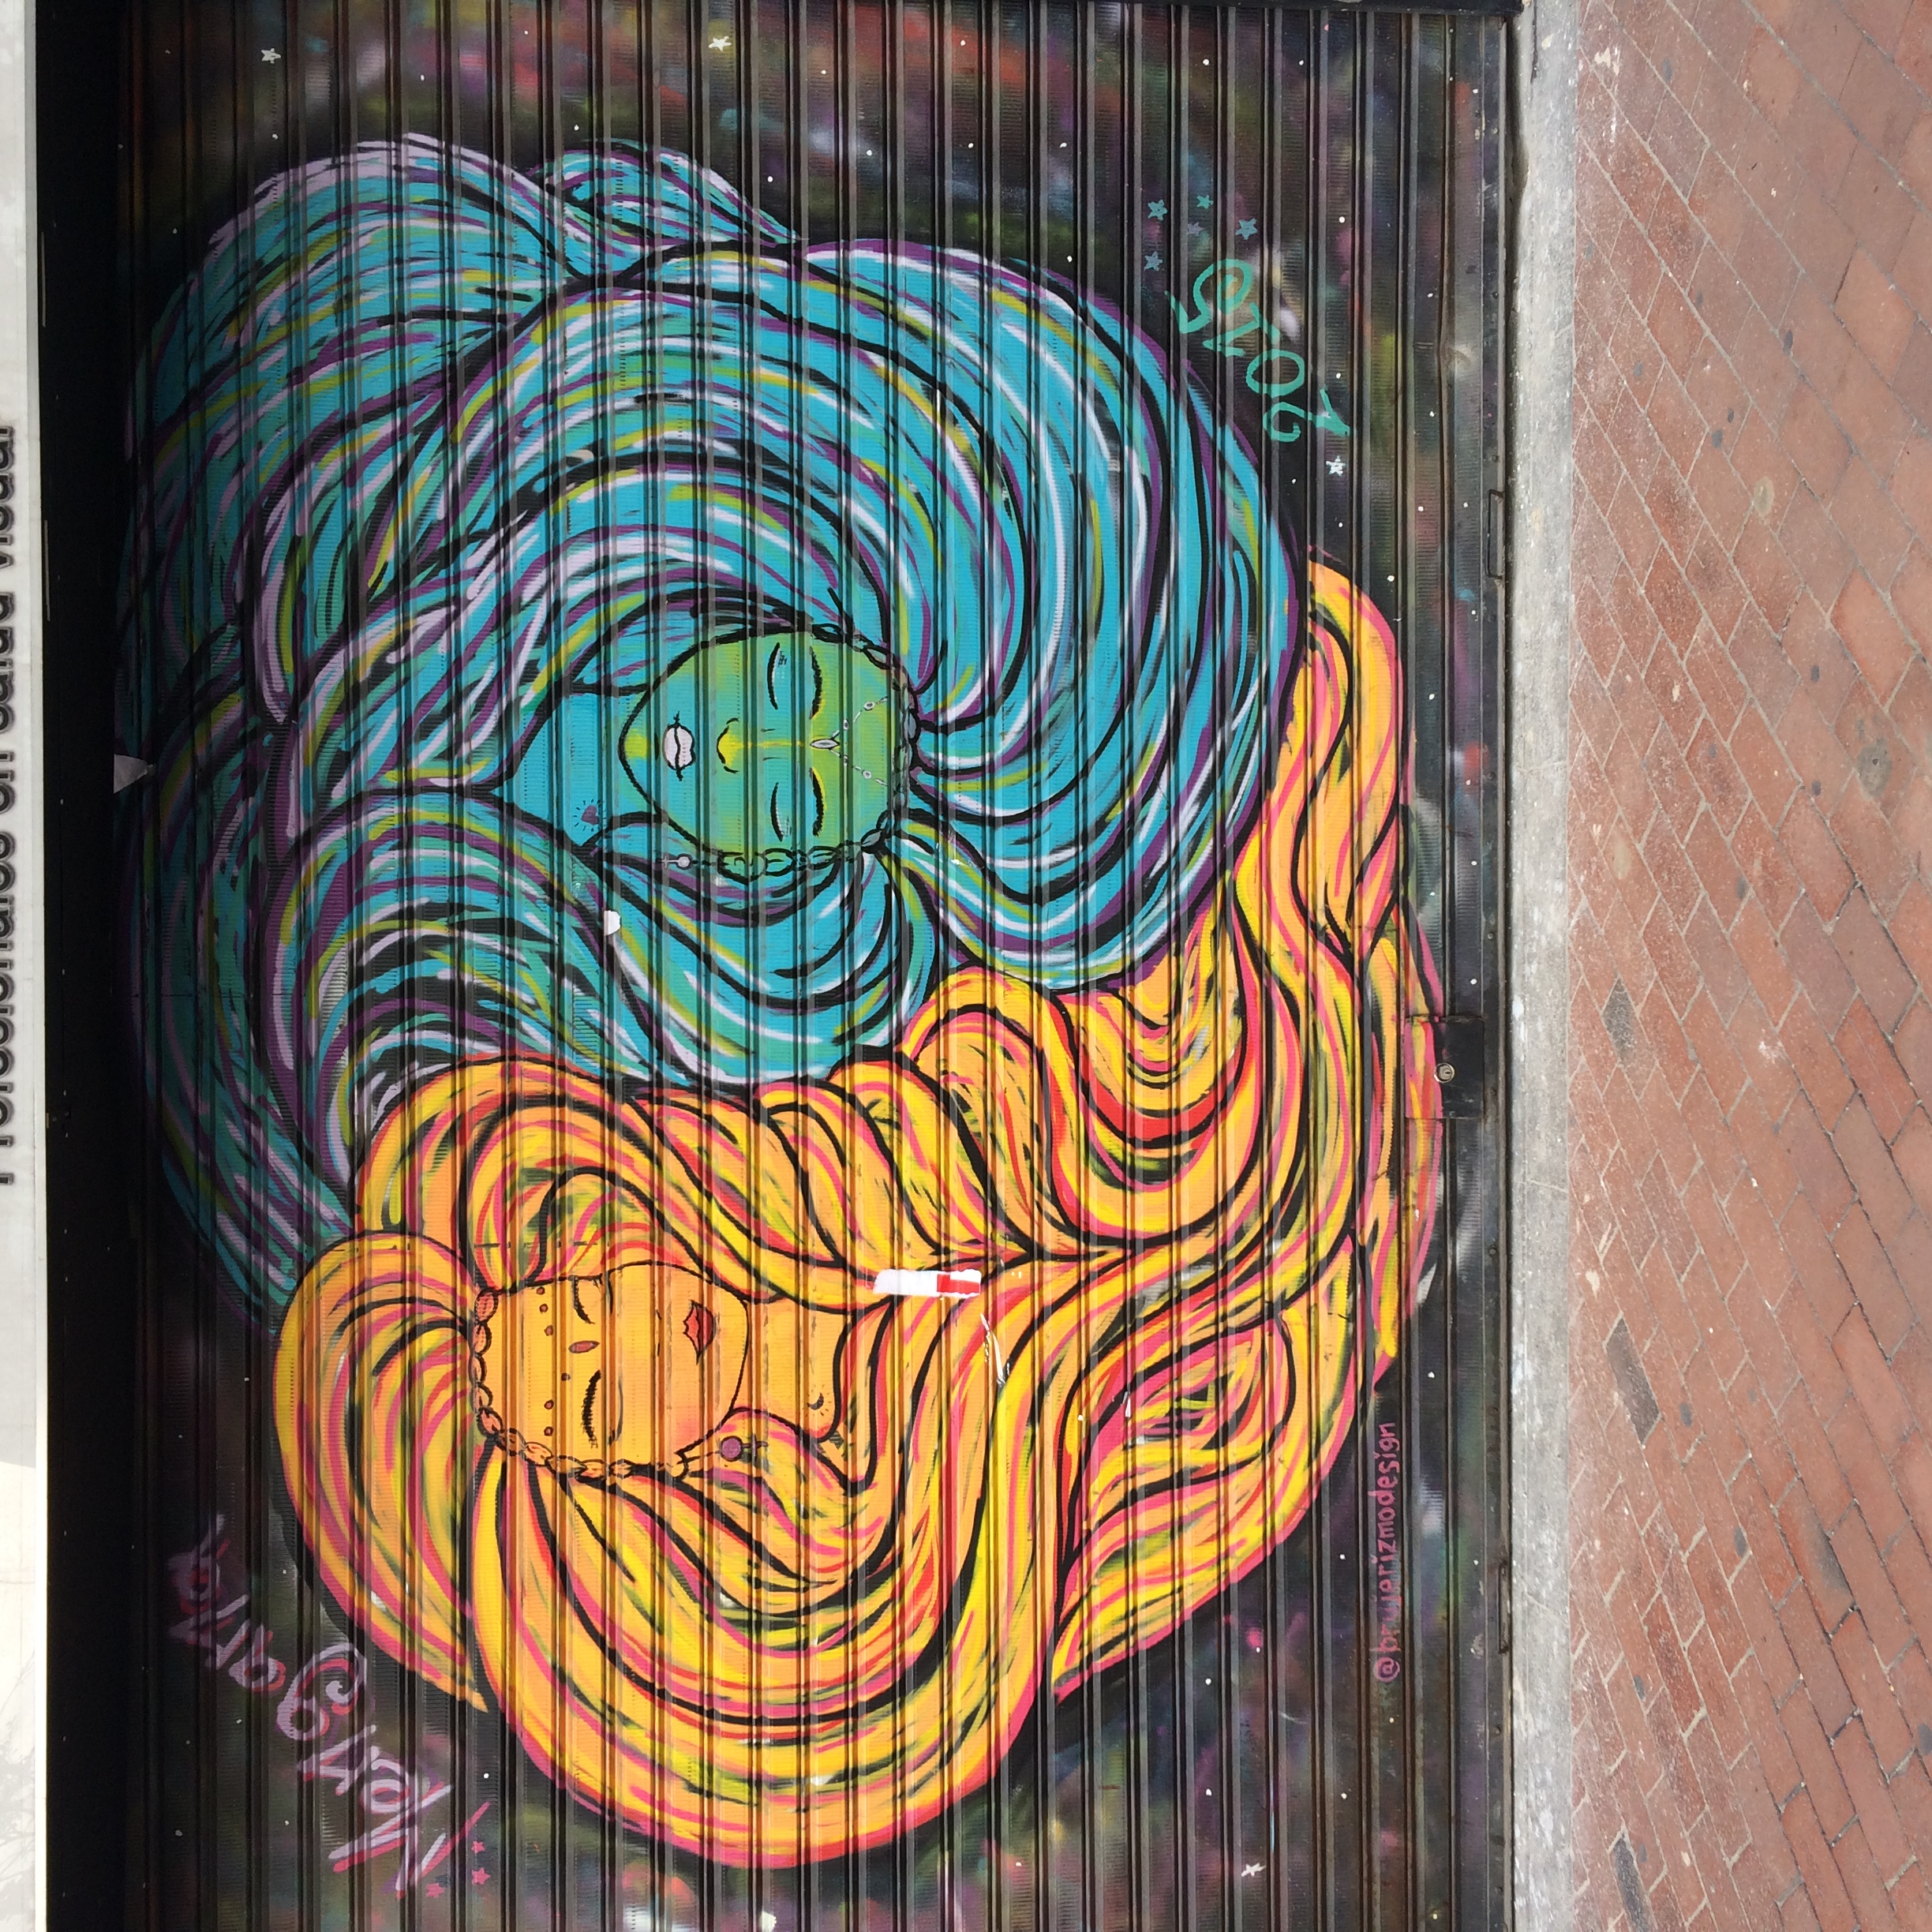
\includegraphics[width=.25\linewidth, angle=270,origin=c]{./graffitti/mujeres.JPG}} &\begin{itemize}
 \item composición (yin/yang) 
 \item mensaje feminista
 \item estilo figurativo
 \item colectivo de modas
 \item @brujerismodesign
 \item no hay anonimidad 
 \end{itemize}	
 
 &  \raisebox{-\totalheight}{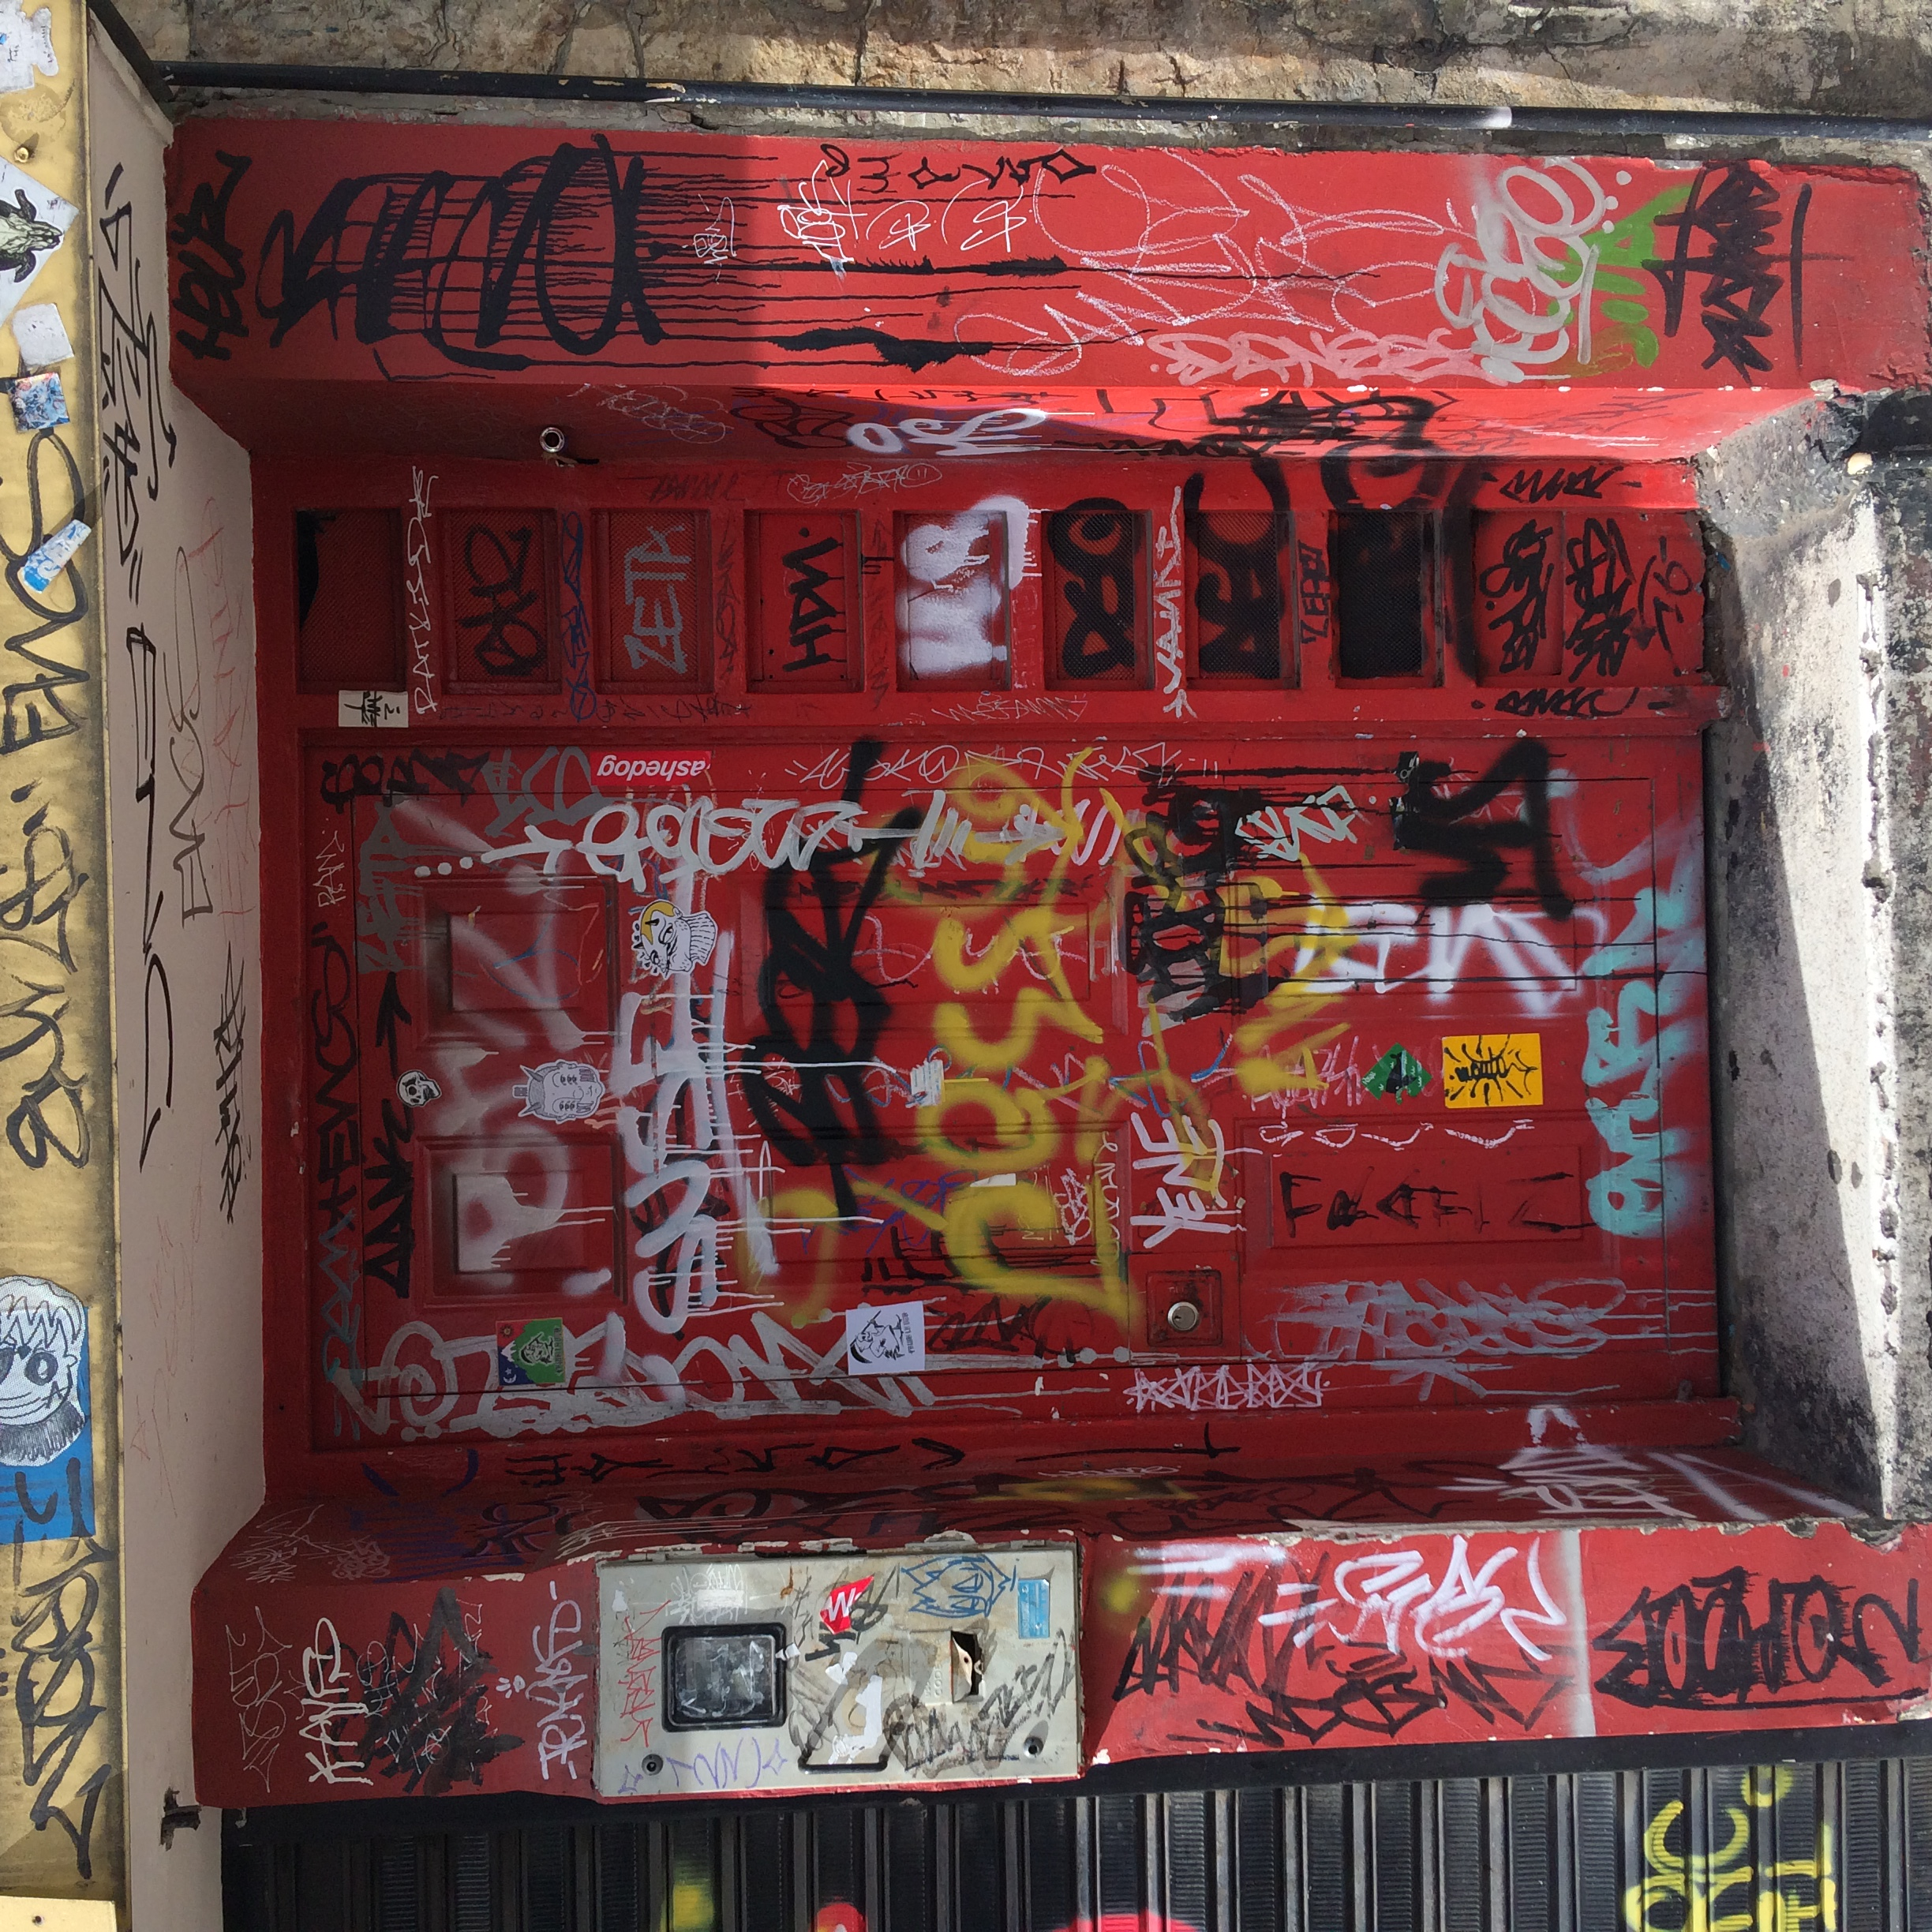
\includegraphics[width=.25\linewidth, angle=270,origin=c]{./graffitti/gffti3.JPG}} &\begin{itemize}
 \item abuso de propiedad abandonada 
 \item se sobrescriben las firmas
 \item rapidez
 \item presencia de pegatinas
 \item proximidad al vandalismo 
 \end{itemize}	
 \\
\hline
\raisebox{-\totalheight}{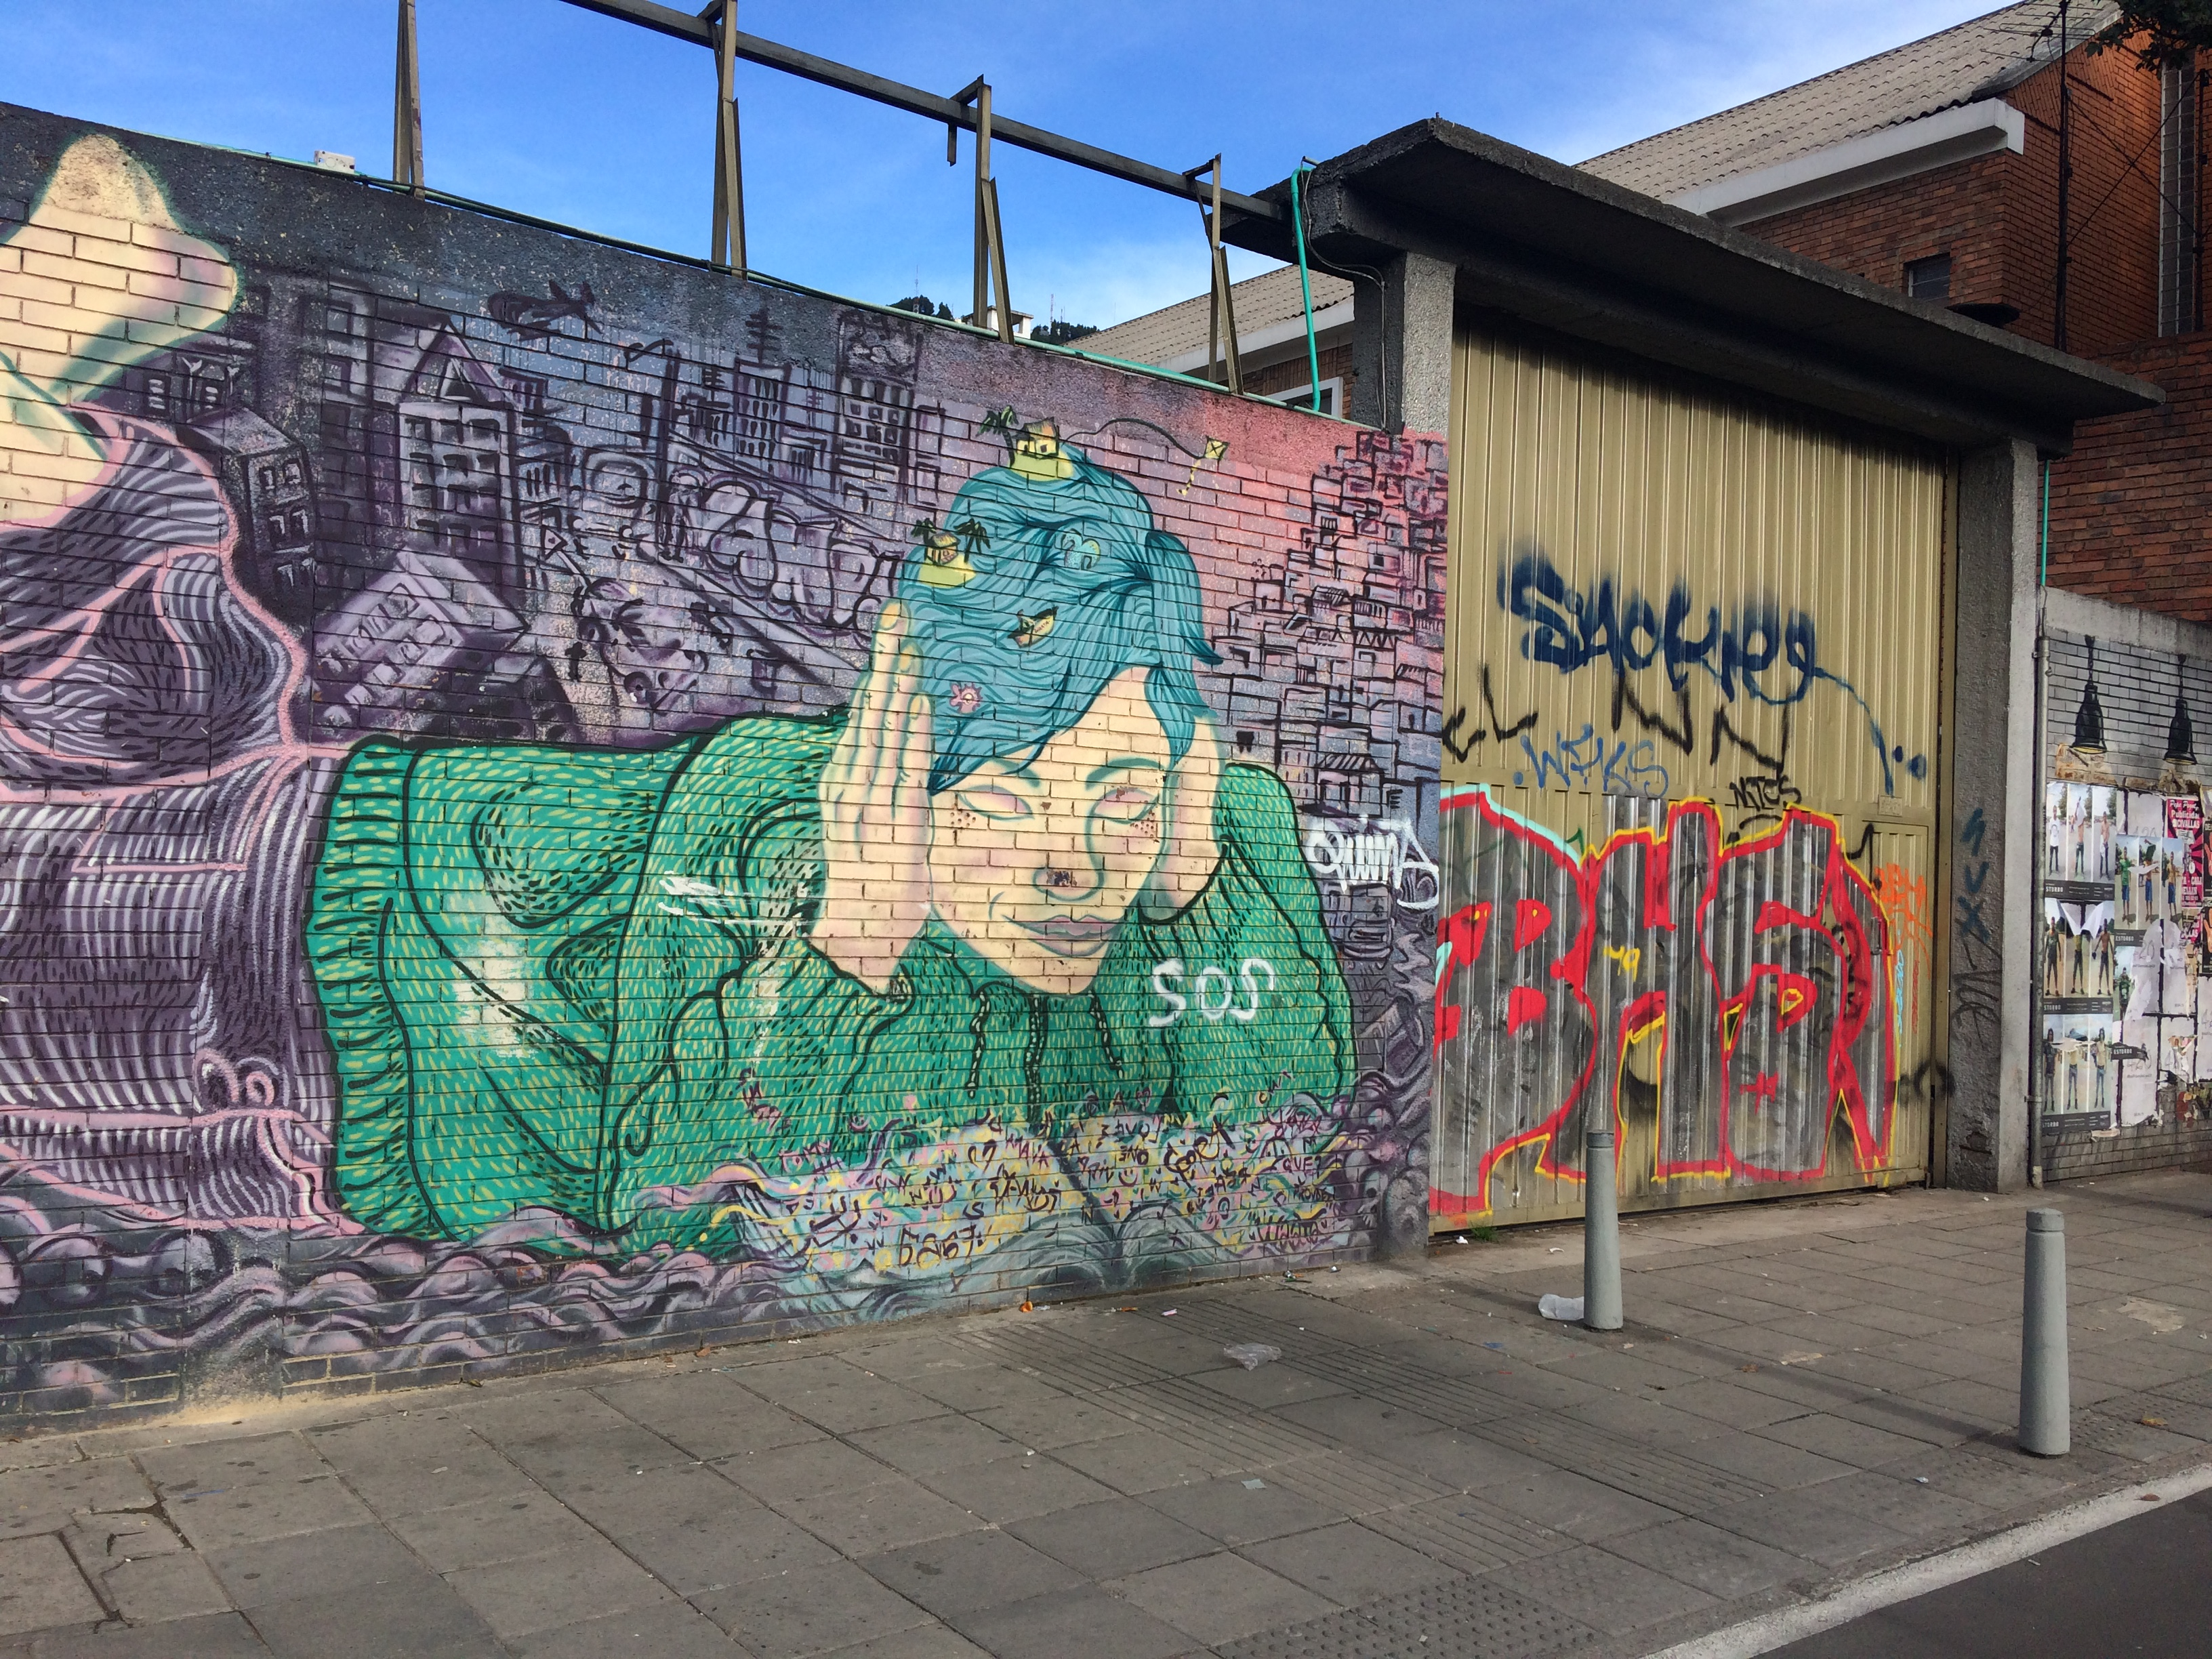
\includegraphics[width=.25\linewidth, angle=0,origin=c]{./graffitti/mural_chapinero.JPG}} & \small\begin{itemize}
\item composición compleja
 \item la ciudad amenaza a joven
 \item la "cultura" como salida
 \item intención muralista
 \item espacio entremezclado con graffitti
 \end{itemize}	
 &
  \raisebox{-\totalheight}{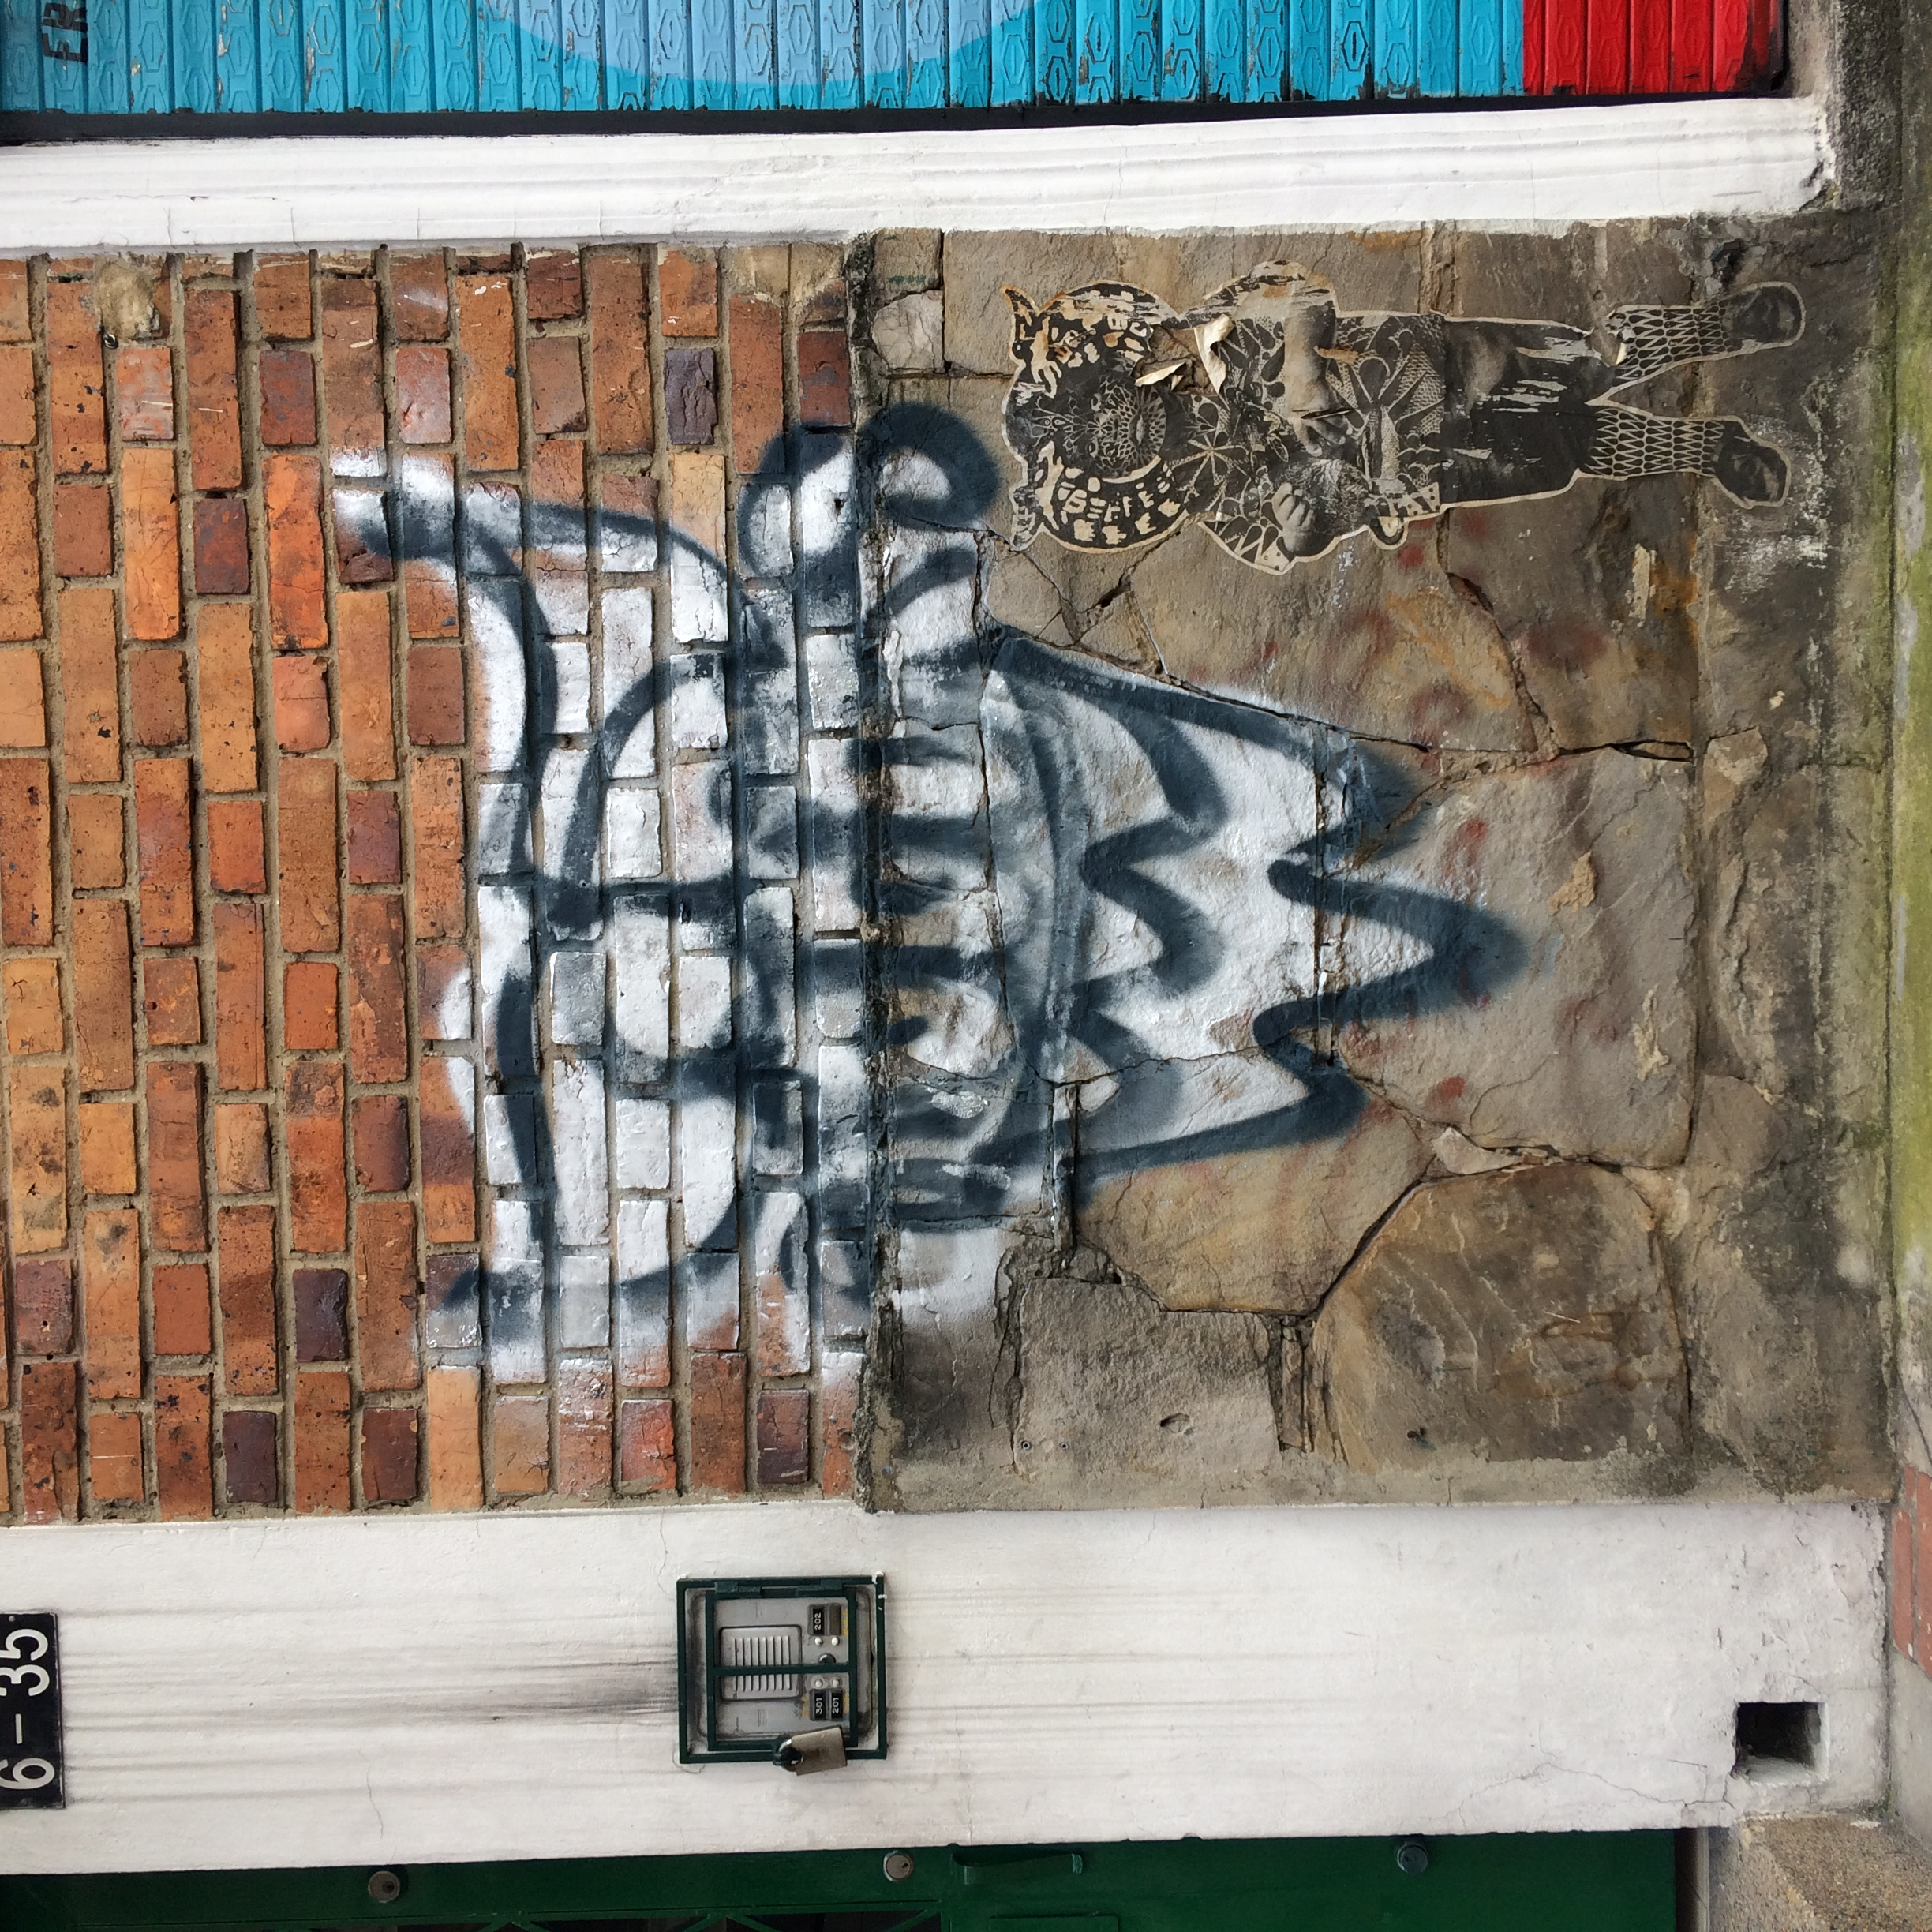
\includegraphics[width=.25\linewidth, angle=270,origin=c]{./graffitti/gffti4.JPG}} &
  \small\begin{itemize}
 \item tag extraño 
 \item forma arbitraria (ilegible)
 \item fondo blanco (mayor composición)
 \item no hay saturación alrededor
 \end{itemize}	
\\
\hline
\raisebox{-\totalheight}{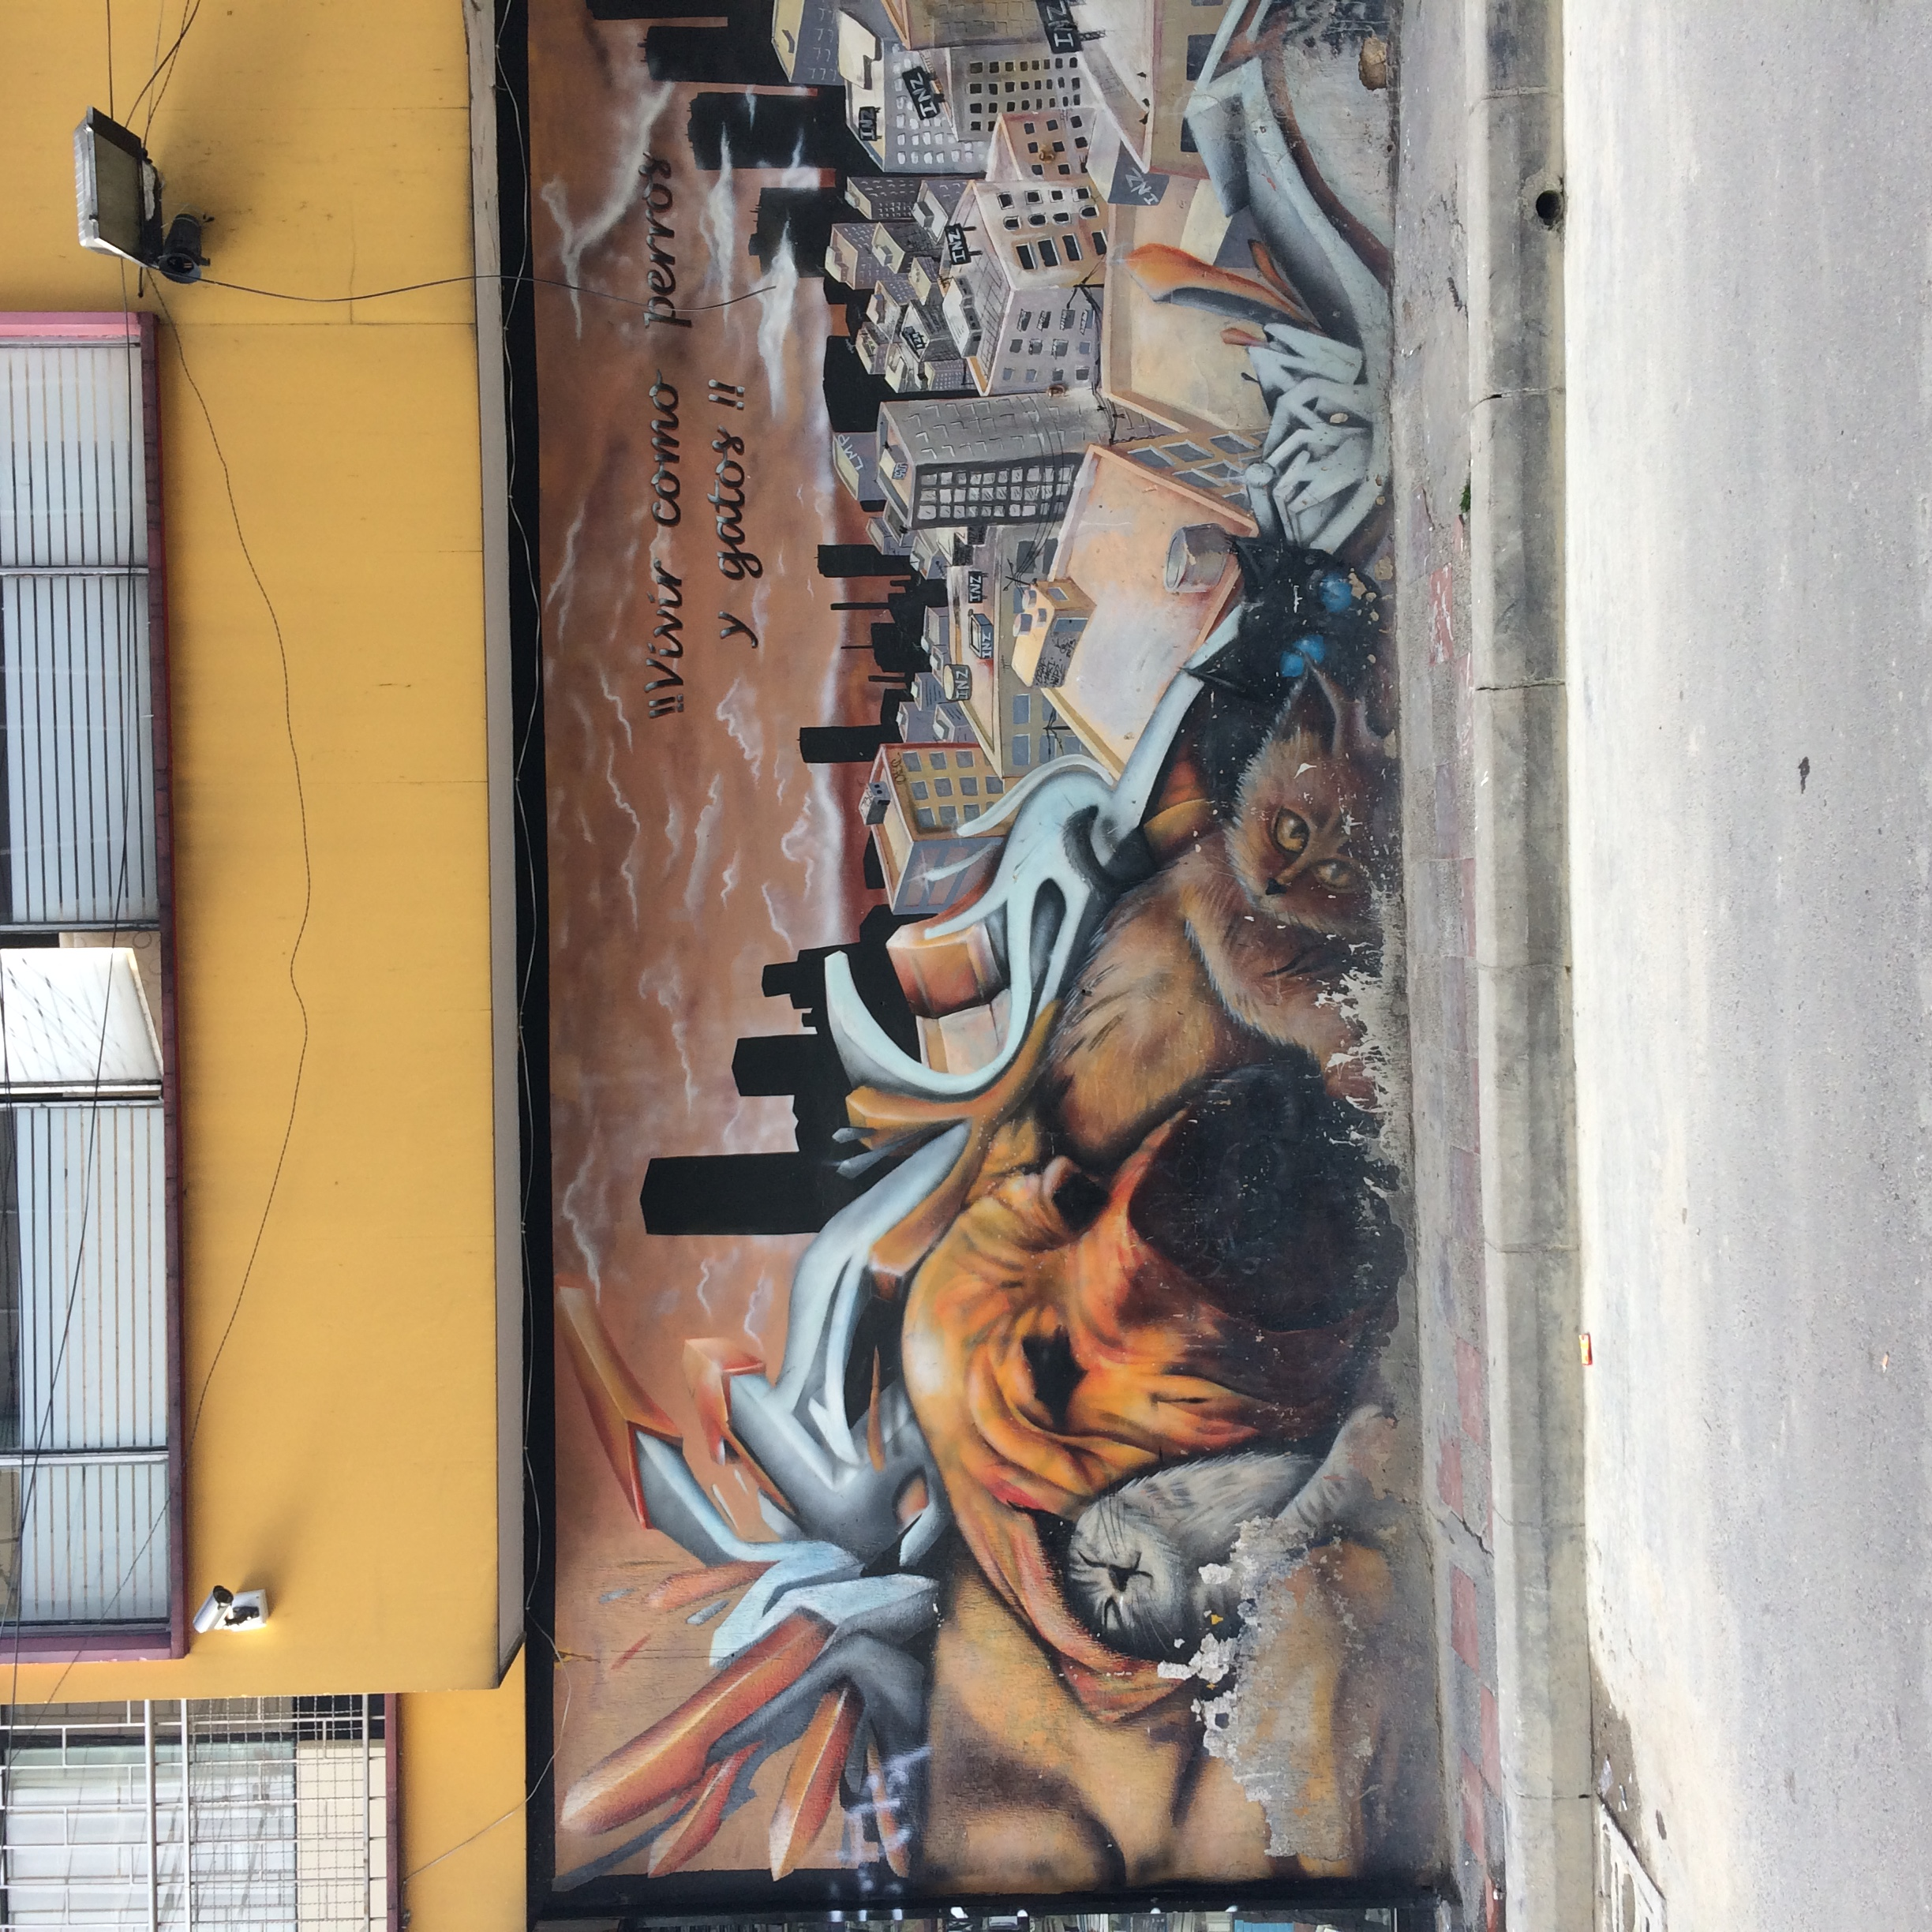
\includegraphics[width=.25\linewidth, angle=270,origin=c]{./graffitti/perros.JPG}} & \begin{itemize}
 \item repudio a la ciudad 
 \item mensaje social y animalista
 \item firma "Inz" reiteradamente
 \item  intención muralista
 \item estilo figurativo 
 \end{itemize}	
&
\raisebox{-\totalheight}{
\includegraphics[width=.25\linewidth, angle=270,origin=c]{./graffitti/gffti5.JPG}} &\begin{itemize}
 \item difícil clasificación
 \item tag de Franco 
 \item marcar territorio 
 \item técnica más pulida que otros tags
 \item tiene página de internet 
 \item no hay anonimidad
 \end{itemize}	
 \\
\hline
\end{longtable}
\end{center}


% Emacs 25.3.50.1 (Org mode 8.2.10)
\end{document}